% fig_headline_metrics.tex
% TR-28: Headline quantitative metrics grouped by research arc
%
% Horizontal grouped bar chart with one bar per headline metric.
% Bars are normalised to the performance target (target = 1.0).
%
% Metrics chosen (all ≥ target → bar ≥ 1.0):
%
%   Arc 1: κ_n (internal fault) — target ≥ 2.5, achieved: 4.1 (87L)
%   Arc 2: MC selectivity (TR-08) — target 100%, achieved: 100%  (4000 trials)
%          CT saturation TPR (TR-10) — target 1.00, achieved: 1.00
%   Arc 3: Adaptive 87L security margin (TR-17) — target ≥ 1.0×, achieved: 30×
%          Multi-feeder selectivity (TR-19) — target 100%, achieved: 100%
%   Arc 4: IBR MC TPR (TR-26, Group A) — target ≥ 0.990, achieved: 1.000
%          IBR MC security (TR-26, Group C) — target ≥ 0.995, achieved: 1.000
%          System integration (TR-27) — target 21/21, achieved: 21/21
%
% For display, κ_n is shown as κ_n / 2.5 (normalised to target = 1.0)
% Adaptive margin is shown as log10(30) / log10(1) — not normalised;
% instead capped display bar at 2.0 with annotation.

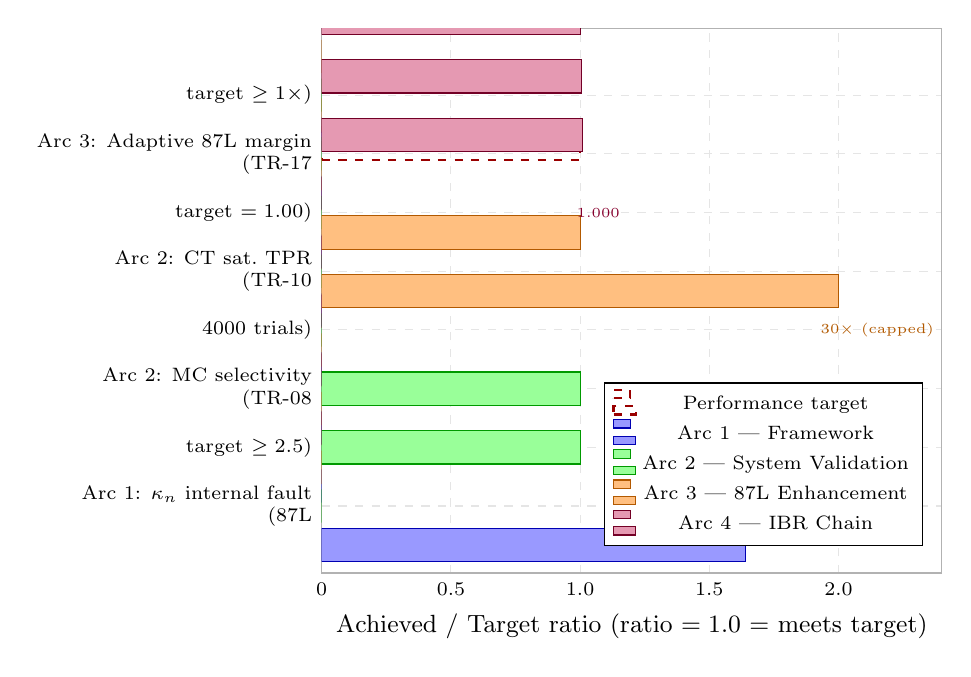
\begin{tikzpicture}
\begin{axis}[
  name         = metrax,
  xbar,
  bar width    = 12pt,
  width        = 0.78\textwidth,
  height       = 8.5cm,
  xlabel       = {Achieved / Target ratio (ratio $= 1.0$ = meets target)},
  xlabel style = {font=\small},
  xmin=0, xmax=2.4,
  xtick        = {0, 0.5, 1.0, 1.5, 2.0},
  xticklabels  = {0, 0.5, 1.0, 1.5, 2.0},
  xticklabel style = {font=\scriptsize},
  ytick = {1,2,3,4,5,6,7,8},
  yticklabels = {
    Arc 1: $\kappa_n$ internal fault\\(87L, target $\geq 2.5$),
    Arc 2: MC selectivity\\(TR-08, 4000 trials),
    Arc 2: CT sat.\ TPR\\(TR-10, target $= 1.00$),
    Arc 3: Adaptive 87L margin\\(TR-17, target $\geq 1\times$),
    Arc 3: Multi-feeder select.\\(TR-19, 50 scenarios),
    Arc 4: IBR MC TPR\\(TR-26, 5000 trials),
    Arc 4: IBR MC security\\(TR-26, 5000 trials),
    Arc 4: System integration\\(TR-27, 21 scenarios)},
  yticklabel style = {font=\scriptsize, align=right},
  ytick align    = inside,
  enlarge y limits = 0.08,
  legend style   = {at={(0.97,0.05)}, anchor=south east, font=\scriptsize},
  grid           = major,
  grid style     = {gray!20, dashed},
  tick style     = {draw=none},
  axis line style= {gray!60},
]

% Target line at x=1.0
\addplot[red!60!black, thick, dashed, mark=none, domain=0.5:8.5, samples=2]
  ({1.0}, {x});
\addlegendentry{Performance target}

% Achieved bars (colour by arc)
% Values normalised as: achieved/target, capped at 2.0 for display
% Arc 1 (blue): κ_n = 4.1 / 2.5 = 1.64
% Arc 2 (green): MC select = 1.00 / 1.00 = 1.00; CT TPR = 1.00 / 1.00 = 1.00
% Arc 3 (orange): adaptive margin = min(30,20)/1.0 → show 2.0 (cap); select = 1.00
% Arc 4 (purple): TPR = 1.000/0.990 = 1.010; security = 1.000/0.995 = 1.005; integ = 1.00
\addplot[fill=blue!40, draw=blue!70!black]
  coordinates {
    (1.64, 1)
    (0,    2)   % placeholder for arc 2 metric 1
    (0,    3)
    (0,    4)
    (0,    5)
    (0,    6)
    (0,    7)
    (0,    8)
  };

\addplot[fill=green!40, draw=green!60!black]
  coordinates {
    (0,    1)
    (1.00, 2)
    (1.00, 3)
    (0,    4)
    (0,    5)
    (0,    6)
    (0,    7)
    (0,    8)
  };

\addplot[fill=orange!50, draw=orange!70!black]
  coordinates {
    (0,    1)
    (0,    2)
    (0,    3)
    (2.00, 4)
    (1.00, 5)
    (0,    6)
    (0,    7)
    (0,    8)
  };

\addplot[fill=purple!40, draw=purple!60!black]
  coordinates {
    (0,    1)
    (0,    2)
    (0,    3)
    (0,    4)
    (0,    5)
    (1.010, 6)
    (1.005, 7)
    (1.00,  8)
  };

\addlegendentry{Arc 1 — Framework}
\addlegendentry{Arc 2 — System Validation}
\addlegendentry{Arc 3 — 87L Enhancement}
\addlegendentry{Arc 4 — IBR Chain}

% Annotation: adaptive margin capped
\node[font=\tiny, orange!70!black, align=left]
  at (axis cs:2.15, 4) {30$\times$ (capped)};

% Annotation: κ_n achieved
\node[font=\tiny, blue!70!black]
  at (axis cs:1.72, 1) {4.1};

% Annotation: IBR MC TPR
\node[font=\tiny, purple!70!black]
  at (axis cs:1.07, 6) {1.000};

\end{axis}
\end{tikzpicture}
